\documentclass[12pt, oneside]{article} 
\usepackage{amsmath, amsthm, amssymb, wasysym, verbatim, bbm, color, geometry}
\usepackage{amsfonts}
\usepackage{csquotes}
\usepackage{polski}
\usepackage[polish]{babel}
\usepackage[nottoc]{tocbibind}
\usepackage{caption}
\usepackage{subcaption}
\usepackage{float}
\usepackage{graphicx}
\usepackage{circuitikz}
\usepackage{listings}
\usepackage{subcaption}
\usepackage{pgffor}
\usepackage{grffile} % Handles special characters in filenames



\captionsetup[subfigure]{labelformat=simple, labelsep=colon}
\renewcommand\thesubfigure{(\alph{subfigure})} % Adds parentheses around letters


\definecolor{codegreen}{rgb}{0,0.6,0}
\definecolor{codegray}{rgb}{0.5,0.5,0.5}
\definecolor{codepurple}{rgb}{0.58,0,0.82}
\definecolor{backcolour}{rgb}{0.95,0.95,0.92}

\lstdefinestyle{mystyle}{
    backgroundcolor=\color{backcolour},   
    commentstyle=\color{codegreen},
    keywordstyle=\color{magenta},
    numberstyle=\tiny\color{codegray},
    stringstyle=\color{codepurple},
    basicstyle=\ttfamily\footnotesize,
    breakatwhitespace=false,         
    breaklines=true,                 
    captionpos=b,                    
    keepspaces=true,                 
    numbers=left,                    
    numbersep=5pt,                  
    showspaces=false,                
    showstringspaces=false,
    showtabs=false,                  
    tabsize=2
}
\lstset{style=mystyle}

% \ctikzset{current arrow scale=1.5} 
\usepackage{hyperref} % Loads the hyperref package for hyperlinks
\usepackage{enumitem}
\usepackage{tikz}
\usepackage{pgfplots}
\usepackage[T1]{fontenc}
\usepackage{algorithm}
\usepackage{algpseudocode}
\usepackage{amsfonts}
\usepackage{mathbbol}
% Make underscore safe in file paths
% \catcode`\_=12
% \def_#1{\sb{\mathrm{#1}}}


\pgfplotsset{compat=1.18} % Set the compatibility level for pg
\usetikzlibrary{shapes.geometric, arrows, positioning, fit, backgrounds}

\hypersetup{
    colorlinks=true,
    linkcolor=blue,
    citecolor=cyan,
    urlcolor=blue!60,
    breaklinks=true,
}

\newcommand{\workSource}[2]{Text available at: \href{#1}{#2}}
\DeclareMathSizes{12}{12}{10}{8}
\makeatletter
\renewcommand\normalsize{%
\@setfontsize\normalsize{12pt}{13.5pt}% Will look incredibly crabbed if line height is too small
\abovedisplayskip 10\p@ \@plus2\p@ \@minus5\p@%
\abovedisplayshortskip \z@ \@plus2\p@%
\belowdisplayshortskip 5\p@ \@plus2\p@ \@minus3\p@%
\belowdisplayskip \abovedisplayskip%
\let\@listi\@listI%
}
\normalsize  
\makeatother

\newcommand{\der}{{\rm d}}
\newcommand{\R}{\mathcal{R}}
\newcommand{\C}{\mathcal{C}}
\newcommand{\M}{\mathcal{M}}
\newcommand{\G}{\mathcal{G}}
\newcommand{\Ron}{R_{\rm ON}}
\newcommand{\Roff}{R_{\rm OFF}}
\newcommand{\von}{V_{\rm ON}}
\newcommand{\voff}{V_{\rm OFF}}
\newcommand{\q}{q}
\newcommand{\ua}{v}
\newcommand{\ia}{i}
\newcommand{\phia}{\varphi}
\newcommand{\xw}{x}
\newcommand{\dert}[1]{\frac{{\rm d} {#1}}{{\rm d} t} }
\newcommand{\inv}[1]{\frac{1}{#1} }
\newcommand{\equal}{=}


\usepackage[style=numeric, 
            backend=biber,
           ]{biblatex}
           
\addbibresource{bibliography.bib} % Replace with your .bib file name

\geometry{
 a4paper,
 total={170mm,257mm},
 left=20mm,
 top=20mm,
}
% \usepackage{fontspec}
% \setmainfont[]{Palatino}

\newcommand{\Cdot}{\boldsymbol{\cdot}}

\newtheorem{thm}{Theorem}
\newtheorem{defn}{Definition}
\newtheorem{conv}{Convention}
\newtheorem{rem}{Remark}
\newtheorem{lem}{Lemma}
\newtheorem{cor}{Corollary}


\title{Pomiary charakterystyk memrystorów}
\author{Karol Bednarz
}
% \date{Rok akademicki 2024--2025}
\date{\today}

\begin{document}

\maketitle
\tableofcontents


\section{Wstęp}
Schemat pomiarowy oraz zdjęcie stanowiska pomiarowego zamieszczono na rysunkach \ref{fig:schemat} oraz \ref{fig:stanowisko}.


\begin{figure}[H]
    \centering
    \begin{subfigure}[b]{0.4\textwidth}
        \centering
        \includegraphics[width=\textwidth]{figures/diagram.pdf}
        \caption{}
        \label{fig:schemat} 
    \end{subfigure}
      \begin{subfigure}[b]{0.5\textwidth}
        \centering
        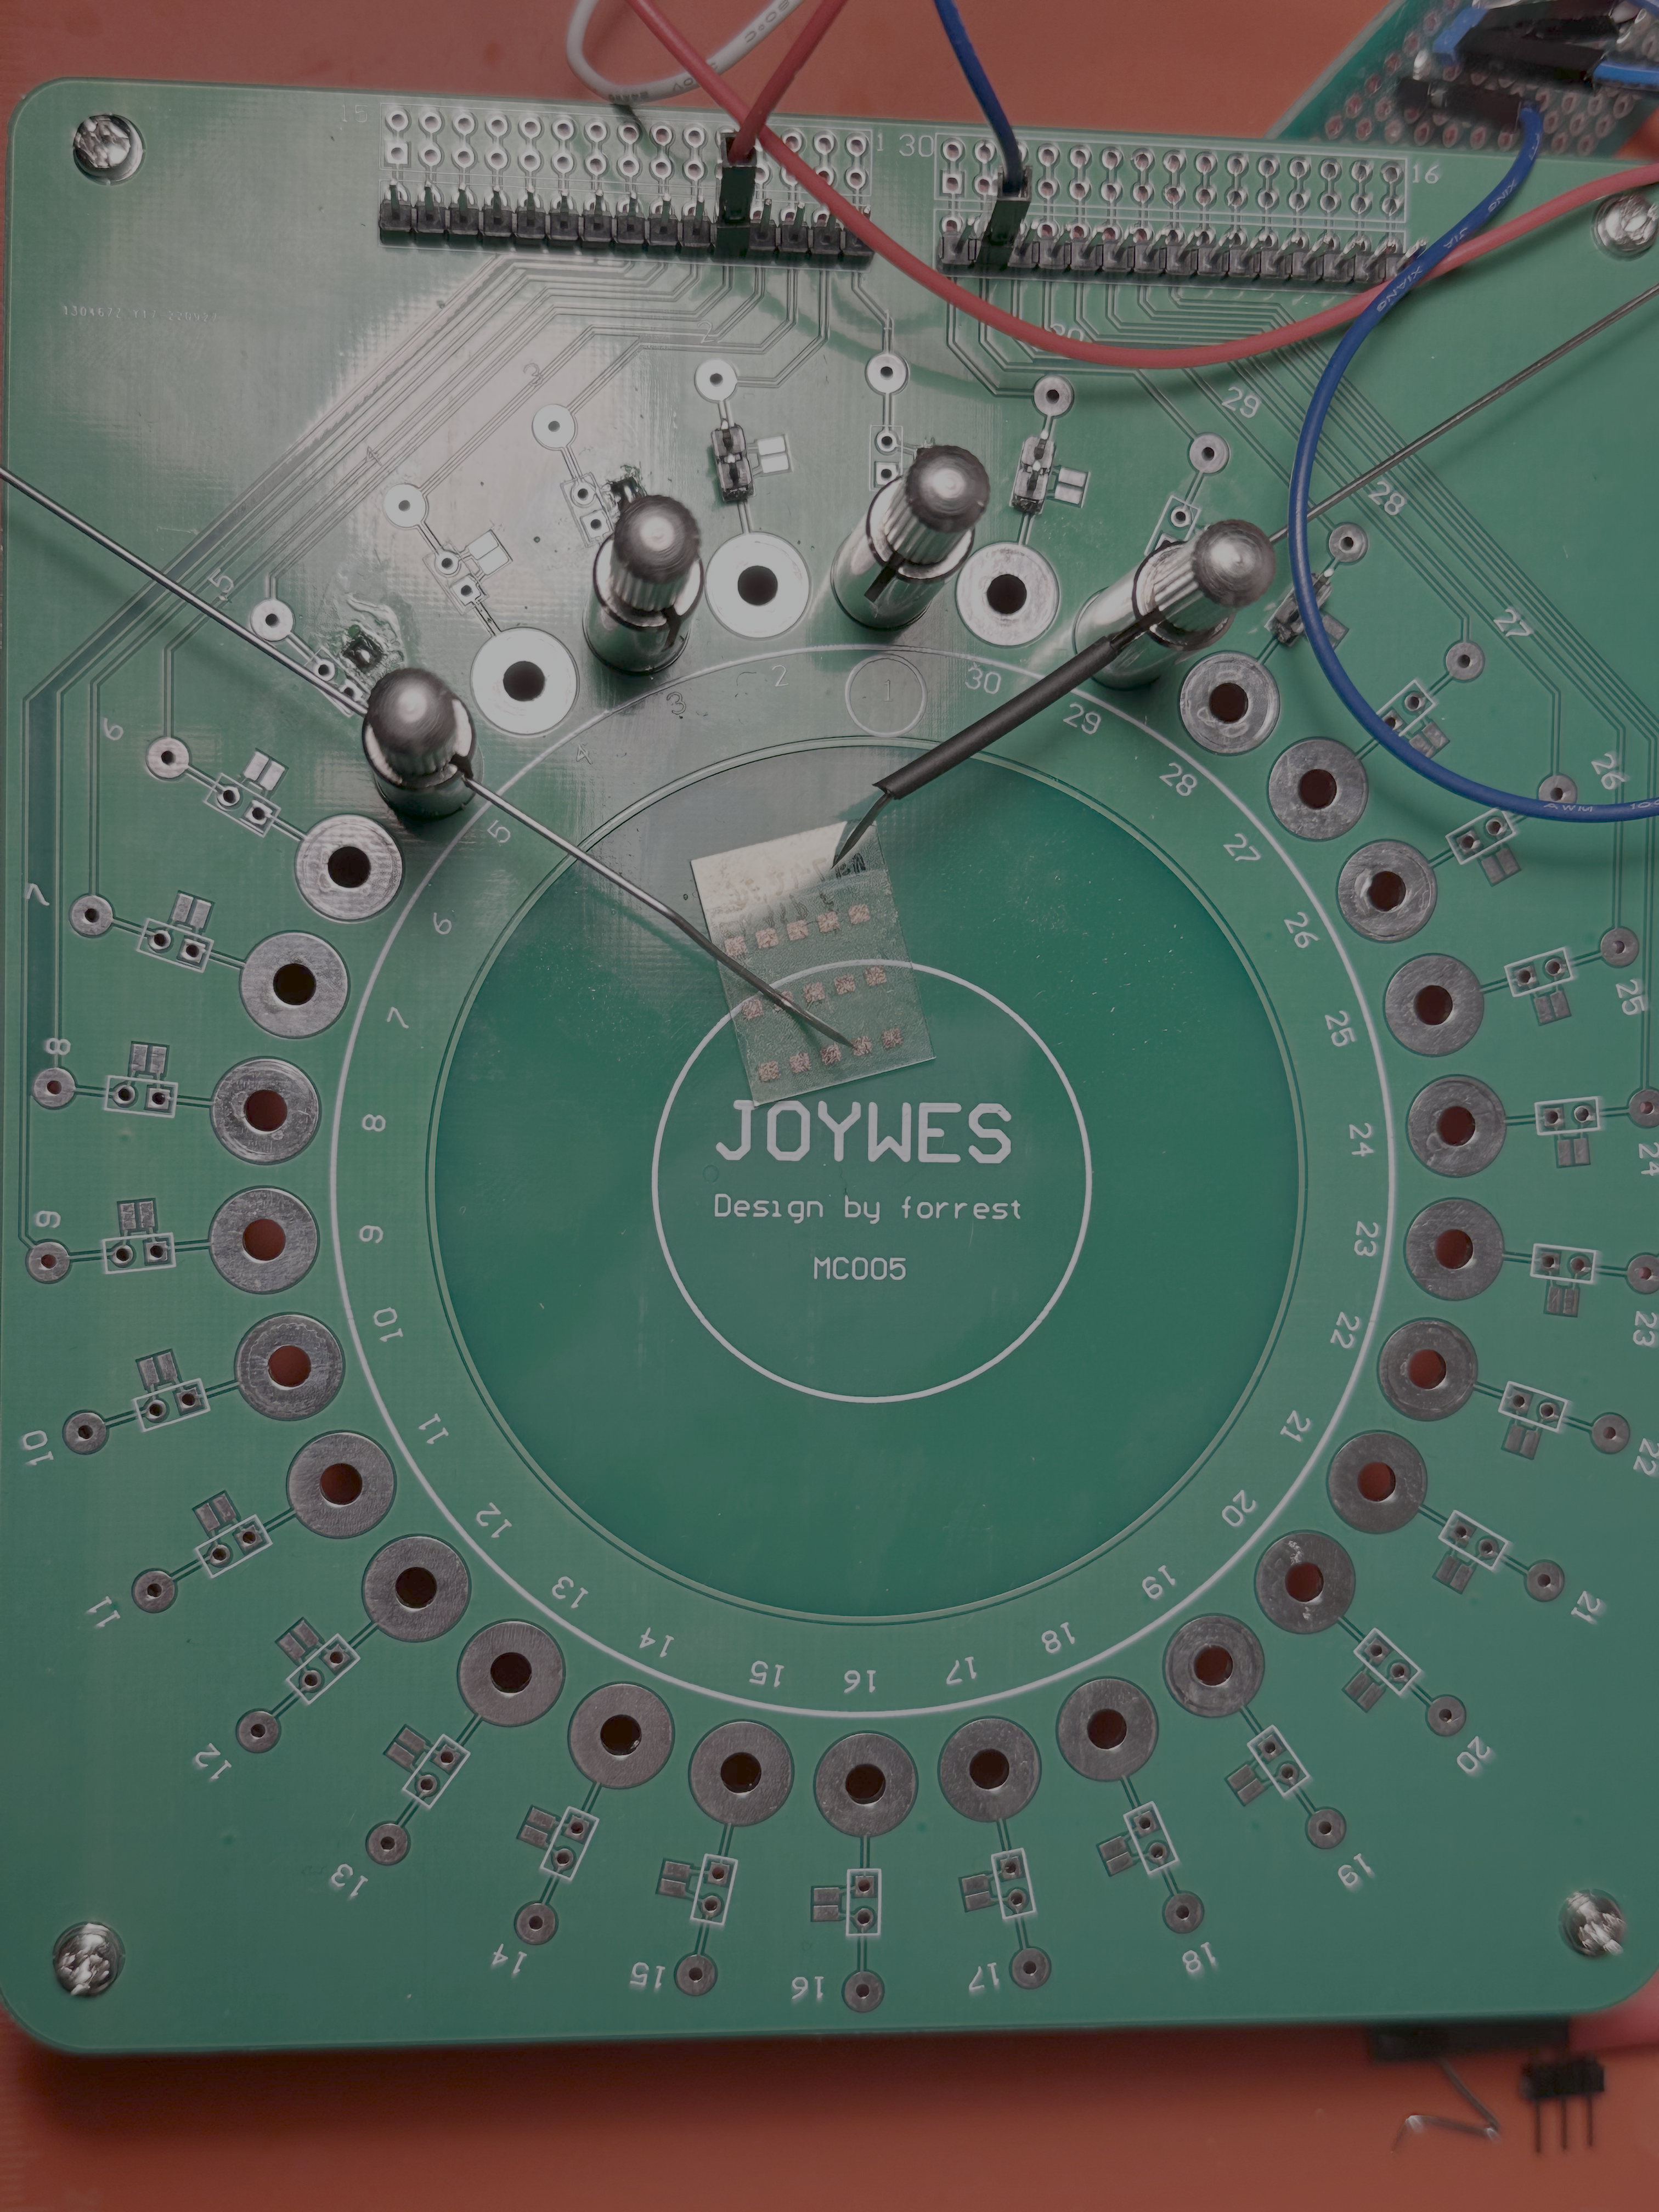
\includegraphics[height=\textwidth, angle=90]{figures/stanowisko.png}
        \caption{}
        \label{fig:stanowisko} 
    \end{subfigure}
    % \hfill
    \caption{\subref{fig:schemat} Schemat pomiarowy oraz \subref{fig:stanowisko} zdjęcie stanowiska pomiarowego.}
    \label{fig:diagram}
\end{figure}
W badaniach zastosowano kartę pomiarową Analog Discovery 3 firmy Digilent, która umożliwia generowanie sygnałów oraz ich akwizycję. Generacja sygnałów realizowana była za pomocą dedykowanej aplikacji z interfejsem graficznym, opracowanej przy użyciu oficjalnego API WaveForms SDK. Proces akwizycji danych przeprowadzono w taki sposób, aby dla każdego okresu napięcia wejściowego zarejestrować 1000 próbek napięcia wyjściowego. W układzie pomiarowym zastosowano rezystor o wartości \(R_s = 0{.}1\,\text{k}\Omega\). Dla kazdego zestawu parametrów sygnału wejściowego (częstotliwość, amplituda, wartość offsetu) przeprowadzono pomiary dla 120 okresów.

\section{Wnioski}

\subsection{Charakter pracy memrystorów}
Większość badanych memrystorów wykazuje zachowanie zbliżone do \textbf{rezystancji nieliniowych} zamiast klasycznego efektu memrystywnego z wyraźną pętlą histerezy. Tylko w nielicznych przypadkach na wykresach wartości średniej obserwuje się charakterystyczną pętlę histerezy.

\subsection{Wpływ częstotliwości na histerezę}
\begin{itemize}
    \item {Najwyraźniejsza pętla histerezy} występuje przy {$f = 20$ Hz},
    \item Przy wyższych częstotliwościach (100 Hz, 1000 Hz, 2000 Hz) pętla histerezy jest słabo widoczna lub nie występuje,
\end{itemize}

\subsection{Dynamika zmian rezystancji}
Pomimo słabej widoczności pętli histerezy przy wyższych częstotliwościach, w wielu przypadkach obserwuje się {zmianę rezystancji elementu} (widoczne wypełnienie części płaszczyzny na wykresach). Istotne jest, że {zmiany te nie dokonują się w ciągu jednego okresu}, co sugeruje powolniejszą dynamikę procesów zachodzących w memrystorze w porównaniu z częstotliwością wymuszenia.





\section{Pomiary}

W niniejszej sekcji przedstawiono wyniki pomiarów przeprowadzonych dla różnych parametrów sygnału wejściowego. Wyniki zostały zaprezentowane w formie graficznej, w pierszym wierszu gdzie wykresy umieszczone po lewej stronie ilustrują pętle histerezy w domeni \(v_m - i_m\) wraz z uśrednioną charakterystyką statyczną. Wykresy znajdujące się po prawej stronie przedstawiają przebiegi czasowe napięcia wejściowego \(v_{\rm s}\) oraz napięcia na memrystorze \(v_m\). Na wykresach czasowych poszczególne okresy sygnału zostały oznaczone punktami, natomiast linia ciągła przedstawia przebieg uśredniony wszystkich zarejestrowanych okresów. W drugim weirszu punkty pomiarowe zostały pokoloryzowane w zależności od numeru okresu, co pozwala na obserwację ewolucji charakterystyki memrystora w czasie.


Jako, że otrzymano dużą liczbę wykresów, w niniejszym dokumencie zamieszczono jedynie wybrane przykłady ilustrujące wpływ poszczególnych parametrów sygnału wejściowego na charakterystyki memrystora. Pełny zestaw wyników pomiarów wraz z plikami \texttt{*.csv} dostępny jest w repozytorium pod linkiem: \href{https://drive.google.com/drive/folders/1UvOOOwlVyftE5LcNZPL52J6Lj1X7XBaA}{[drive]}. Rozbito również wyniki pomiarów na dwa oddzielne katalogi, ze względu na otrymane dwa różne typy memrystorów. 

Pozycje memrystorów w układzie zostały oznaczone wg. schematu na rusunku \ref{fig:matrix}.
\begin{figure}[H]
    \centering
    \includegraphics[width=0.6\textwidth]{figures/macierz.pdf}
    \caption{Schemat numeracji memrystorów w układzie pomiarowym.}
    \label{fig:matrix}
\end{figure}

\newcommand{\memposplot}[2]{%
    \begin{figure}[H]
        \centering
        \includegraphics[width=1\textwidth]{#1}
        \caption{Pozycja: #2}
    \end{figure}
}


\subsection{Memrystor w pozycji I (cuaspf)}
\memposplot{./pos_mems/cuaspf/1_1/temp_0.10_100.0_2.5_Sine_1765395574.png}{ (1,1)}
\memposplot{./pos_mems/cuaspf/2_2/temp_0.10_10.0_2.5_Sine_1765396062.png}{ (2,2)}
\memposplot{./pos_mems/cuaspf/2_2/temp_0.10_100.0_2.5_Sine_1765396040.png}{ (2,2)}
\memposplot{./pos_mems/cuaspf/2_2/temp_0.10_1000.0_2.5_Sine_1765396010.png}{ (2,2)}
\memposplot{./pos_mems/cuaspf/2_4/temp_0.10_10.0_2.5_Sine_1765396475.png}{ (2,4)}
\memposplot{./pos_mems/cuaspf/2_4/temp_0.10_100.0_2.5_Sine_1765396456.png}{ (2,4)}
\memposplot{./pos_mems/cuaspf/2_4/temp_0.10_1000.0_2.5_Sine_1765396486.png}{ (2,4)}


\subsection{Memrystor w pozycji II (perwen)}

% \memposplot{./pos_mems/perwen/1_3/temp_0.10_10.0_2.5_Sine_1765400948.png}{(1,3)}
\memposplot{./pos_mems/perwen/1_3/temp_0.10_100.0_2.5_Sine_1765400958.png}{(1,3)}
\memposplot{./pos_mems/perwen/1_3/temp_0.10_1000.0_2.5_Sine_1765400969.png}{(1,3)}
\memposplot{./pos_mems/perwen/1_3/temp_0.10_1000.0_2.5_Sine_1765400983.png}{(1,3)}
\memposplot{./pos_mems/perwen/1_4/temp_0.10_1000.0_2.5_Sine_1765401101.png}{(1,4)}
\memposplot{./pos_mems/perwen/2_0/temp_0.10_10.0_2.5_Sine_1765400160.png}{(2,0)}
\memposplot{./pos_mems/perwen/2_0/temp_0.10_100.0_2.5_Sine_1765400124.png}{(2,0)}
\memposplot{./pos_mems/perwen/2_0/temp_0.10_1000.0_2.5_Sine_1765400135.png}{(2,0)}
\memposplot{./pos_mems/perwen/2_1/temp_0.10_10.0_2.5_Sine_1765401431.png}{(2,1)}
\memposplot{./pos_mems/perwen/2_1/temp_0.10_100.0_2.5_Sine_1765401381.png}{(2,1)}
\memposplot{./pos_mems/perwen/2_1/temp_0.10_1000.0_2.5_Sine_1765401391.png}{(2,1)}




\section{Wyniki pomiarów, bez sprecyzowanej pozycji memrystora}
\subsection{Memrystor I (cuaspf)}

\newcommand{\addplot}[1]{%
    \begin{figure}[H]
        \centering
        \includegraphics[width=1\textwidth]{mem1/hysteresis_plots/#1.png}
        \caption{}
    \end{figure}
}

\addplot{temp_0.10_100.0_2.5_Sine_1764609477}
\addplot{temp_0.10_100.0_2.5_Sine_1764609505}
\addplot{temp_0.10_100.0_2.5_Sine_1764609521}
\addplot{temp_0.10_100.0_2.5_Sine_1764610872}
\addplot{temp_0.10_100.0_2.5_Sine_1764610889}
% \addplot{temp_0.10_100.0_2.5_Sine_1764610895}
\addplot{temp_0.10_100.0_2.5_Sine_1764610907}
\addplot{temp_0.10_100.0_2.5_Sine_1764610913}
\addplot{temp_0.10_100.0_2.5_Sine_1764610921}
\addplot{temp_0.10_100.0_2.5_Sine_1764610940}
\addplot{temp_0.10_100.0_2.5_Sine_1764610949}
\addplot{temp_0.10_100.0_2.5_Sine_1764610960}
% \addplot{temp_0.10_100.0_2.5_Sine_1764610975}
\addplot{temp_0.10_100.0_2.5_Sine_1764611007}
\addplot{temp_0.10_100.0_2.5_Sine_1764611017}
\addplot{temp_0.10_100.0_2.5_Sine_1764611043}
\addplot{temp_0.10_100.0_2.5_Sine_1764611059}
\addplot{temp_0.10_100.0_2.5_Sine_1764611114}
\addplot{temp_0.10_100.0_2.5_Sine_1764611228}
\addplot{temp_0.10_100.0_2.5_Sine_1764611238}
\addplot{temp_0.10_100.0_2.5_Sine_1764611256}


\subsection{Memrystor II (perwen)}


\renewcommand{\addplot}[1]{%
    \begin{figure}[H]
        \centering
        \includegraphics[width=1\textwidth]{mem2/hysteresis_plots/#1.png}
        \caption{}
    \end{figure}
}

\addplot{temp_0.10_20.0_2.5_Sine_1764612711}
\addplot{temp_0.10_20.0_2.5_Sine_1764612727}
\addplot{temp_0.10_100.0_2.5_Sine_1764612227}
\addplot{temp_0.10_100.0_2.5_Sine_1764612236}
% \addplot{temp_0.10_100.0_2.5_Sine_1764612243}
\addplot{temp_0.10_100.0_2.5_Sine_1764612278}
\addplot{temp_0.10_100.0_2.5_Sine_1764612285}
\addplot{temp_0.10_100.0_2.5_Sine_1764612293}
\addplot{temp_0.10_100.0_2.5_Sine_1764612307}
\addplot{temp_0.10_100.0_2.5_Sine_1764612324}
\addplot{temp_0.10_100.0_2.5_Sine_1764612689}
\addplot{temp_0.10_100.0_2.5_Sine_1764612745}
\addplot{temp_0.10_100.0_2.5_Sine_1764612761}
\addplot{temp_0.10_100.0_2.5_Sine_1764612769}
\addplot{temp_0.10_100.0_2.5_Sine_1764612776}
\addplot{temp_0.10_100.0_2.5_Sine_1764612786}
\addplot{temp_0.10_100.0_2.5_Sine_1764612795}
\addplot{temp_0.10_100.0_2.5_Sine_1764612816}
\addplot{temp_0.10_100.0_2.5_Sine_1764612831}
\addplot{temp_0.10_100.0_2.5_Sine_1764612855}
\addplot{temp_0.10_1000.0_2.5_Sine_1764612583}
\addplot{temp_0.10_1000.0_2.5_Sine_1764612590}
\addplot{temp_0.10_1000.0_2.5_Sine_1764612596}
\addplot{temp_0.10_1000.0_2.5_Sine_1764612601}
\addplot{temp_0.10_1000.0_2.5_Sine_1764612605}
\addplot{temp_0.10_1000.0_2.5_Sine_1764612613}
\addplot{temp_0.10_1000.0_2.5_Sine_1764612619}
\addplot{temp_0.10_1000.0_2.5_Sine_1764612627}
\addplot{temp_0.10_2000.0_2.5_Sine_1764612639}

\end{document}
